\documentclass{article}
\usepackage{amsfonts}
\usepackage{amsthm}
\usepackage{amssymb}
\usepackage{amsmath}
\usepackage{graphicx}
\usepackage{subcaption}
\usepackage{xcolor}
\usepackage{mathtools}
\usepackage{ wasysym }
\usepackage{enumerate}
\usepackage{verbatim}

\numberwithin{equation}{section}

\newcommand{\new}[2]{
    \vspace{2mm}
    \noindent
    \textbf{
    \underline{#1}}
    \textit{{#2}}
    \
}

\def\<{{\langle}}
\def\>{{\rangle}}

\DeclarePairedDelimiter\bra{\langle}{\rvert}
\DeclarePairedDelimiter\ket{\lvert}{\rangle}
\DeclarePairedDelimiterX\braket[2]{\langle}{\rangle}{#1\,\delimsize\vert\,\mathopen{}#2}


\newcommand{\textOr}{
    {
        \hspace{5mm}
        \textrm{or}
        \hspace{5mm}
    }
}

\newcommand{\textAnd}{
    {
        \hspace{5mm}
        \textrm{and}
        \hspace{5mm}
    }
}


\newcommand{\textWhere}{
    {
        \hspace{5mm}
        \textrm{where}
        \hspace{5mm}
    }
}



\newcommand{\Ixp}[1]{
    {
        e^{i{#1}}
    }
}



\newcommand{\halfFigure}[1]{
\begin{center}
\includegraphics[width = .5\linewidth]{{#1}}
\end{center}
}

\newcommand{\fullFigure}[1]{
\begin{center}
\includegraphics[width = .9\linewidth]{{#1}}
\end{center}
}

\def\twobytwoMat(#1, #2, #3, #4){
    {
        \begin{bmatrix}
            {#1} & {#2}\\
            {#3} & {#4}
        \end{bmatrix}
    }
}

\def\twobyoneMat(#1, #2){
    {
        \begin{bmatrix}
            {#1}\\
            {#2}
        \end{bmatrix}
    }
}

\def\twobytwoDet(#1, #2, #3, #4){
    {
        \begin{vmatrix}
            {#1} & {#2}\\
            {#3} & {#4}
        \end{vmatrix}
    }
}


\newcommand{\RR}{\mathbb{R}}
\newcommand{\CC}{\mathbb{C}}
\newcommand{\ZZ}{\mathbb{Z}}
\newcommand{\Zpos}{\mathbb{Z}_{pos}}
\newcommand{\NN}{\mathbb{N}}

\newtheorem{theorem}{Theorem}
\newtheorem{proposition}{Proposition}
\newtheorem{lemma}{Lemma}
\newtheorem{corollary}{Corollary}
\newtheorem{remark}{Remark}
\newtheorem{definition}{Definition}
\newtheorem{example}{Example}
\newtheorem{conjecture}{Conjecture}
\newtheorem{question}{Question}

\newcommand{\ch}{\text{ch}}

\begin{document}
\begin{center}
    \Large
    \textbf{Pset 1}

    \large
    Daniel Son
\end{center}

\section*{0) Series Expansions}

Write and memorize the [Taylor]\textsuperscript{1} series expansions for small $x$:

\begin{itemize}
    \item[(A)] $e^x$
    \item[(B)] $\cos x$
    \item[(C)] $\sin x$
    \item[(D)] $(1 + x)^p$
    \item[(E)] $\ln (1 + x)$
\end{itemize}

\begin{proof}[Solution]
    
\end{proof}
\begin{itemize}
    \item[(A)] \begin{eqnarray}
        e^x  \ = \ 1 + x + \frac {x^2} 2 + \cdots
    \end{eqnarray}
    \item[(B)] \begin{eqnarray}
        \cos(x) \ = \ 1 - \frac {x^2} 2 + \frac {x^4} {4!} + \cdots 
    \end{eqnarray}
    \item[(C)] \begin{eqnarray}
        \sin(x) \ = \ x - \frac {x^3} {3!} + \frac {x^5}{5!} + \cdots
    \end{eqnarray}
    \item[(D)] \begin{eqnarray}
        (1 + x)^p \ = \ 1 + px + \frac {p(p - 1)} 2 x^2 + \cdots
    \end{eqnarray}
    \item[(E)] \begin{eqnarray}
        \ln(1 + x) \ = \ x - \frac {x^2}  2 + \frac {x^3} {3} + \cdots
    \end{eqnarray}
\end{itemize}

\section{Problem 1}




\begin{quote}
\textbf{2.17} $\star$ The two equations (t2.36) give a projectile's position $(x, y)$ as a function of $t$. Eliminate $t$ to give $y$ as a function of $x$. Verify Equation (t2.37).
\end{quote}

\begin{equation}
x(t) = v_{x_0} \tau \left( 1 - e^{-t/\tau} \right)
\end{equation}

\begin{equation}
y(t) = \left( v_{y_0} + v_{\text{ter}} \right) \tau \left( 1 - e^{-t/\tau} \right) - v_{\text{ter}} t
\end{equation}

\hfill (t2.36)

\begin{equation}
y = \frac{v_{y_0} + v_{\text{ter}}}{v_{x_0}} x + v_{\text{ter}} \tau \ln \left( 1 - \frac{x}{v_{x_0} \tau} \right)
\end{equation}

\hfill (t2.37)


\begin{proof}[Solution]
    We wish to verify equation (t2.37). We start off by solving 
    for $1 - e^{t/\tau}$ from equation (t2.36). 
    \begin{equation}
        1 - e^{t/\tau} \ = \ 
        \frac {x(t)} {v_{x0} \tau} 
        \ = \ 
        \frac {y(t) + v_{\rm ter} t}{v_{y0}+v_{\rm ter}}\tau
    \end{equation}
    Fiddling with the second equality, we can solve for $y$. 
    \begin{equation}
        y \ = \ \frac {v_{x0} + g \tau} {v_{x0}}x - v_{\rm ter} t
    \end{equation}
    Solve for $-v_{\rm ter}t$ using the first two equality. 
    \begin{equation}
        -v_{\rm ter}t \ = \ \tau v_{\rm ter} \ln\left(1 - \frac x {v_{x0} \tau}\right)
    \end{equation}
    We obtain (t2.37). 
\begin{equation}
        0 \ = \ \frac {v_{x0} + g \tau} {v_{x0}}x + \tau v_{\rm ter} \ln\left(1 - \frac x {v_{x0} \tau}\right)
    \end{equation}
    Also, it is useful to note the following. 
    \begin{equation}
        v_{\rm ter} = \tau g
    \end{equation}
\end{proof}

\textbf{(B)} The range $R$ of a projectile is defined as the (non-zero) value of $x = R$ for which the height $y = 0$. Using length scales $R_{vac} =  2v_{x0}v_{y0}/g$ and $R_{\infty} = v_{x0}\tau$, rewrite Eq. (2.39) in terms of these scales. 
{What is the significance of $R_{\infty}$?}

\begin{equation}
\frac{v_{y_0} + v_{\text{ter}}}{v_{x_0}} R + v_{\text{ter}} \tau \ln \left( 1 - \frac{R}{v_{x_0} \tau} \right) = 0
\end{equation}

\hfill (t2.39)


\begin{proof}[Solution]
    Express $v_{x0}, v_{y_0}$ in terms of $R_{\rm vac}, R_\infty$. 
    \begin{equation}
        v_{x0} \ = \ \frac {R_\infty} \tau \textAnd 
        v_{y0} \ = \ \frac {\tau g R_{\rm vac}}{2 R_\infty}
    \end{equation}
    Plugging in and applying algebraic manipulations yields the following. 
    \begin{equation}\label{eqn:Q1Braw}
        \left(
            \frac {R_{\rm vac} \tau g}{R_\infty 2} + \tau g
        \right)\frac {R}{R_\infty} + \tau^2 g \ln\left(
            1 - \frac R {R_{\infty}}
        \right) \ = \ 0
    \end{equation}
    $R_\infty$ is the length the projectile travels for large $t$. 
    If $t \rightarrow \infty$, 
    \[
    x \ = \ v_{x0}\tau (1- e^{-\infty}) \ \approx \ v_{x0}\tau \ = \ R_\infty
    \]where $\epsilon =t/\tau \approx 0$. 
\end{proof}

\textbf{(C)} The range equation from part (B) can be written in a dimensionless form by using two scaled lengths: $z = R/R_{\infty}$ and $w = R_{vac}/R_{\infty}$. Rewrite the equation in terms of these lengths; you should find that the result is a transcendental function for $z$ as a function of $w$ which you can write in the form $g(z, w) = 0$. Use \textit{Mathematica} or similar to evaluate $z(w)$ for 20 values of $w$ between 0 and 10. You may find some of the following commands to be helpful: \texttt{FindRoot}, \texttt{Do}, \texttt{For}, \texttt{Table}, \texttt{ListPlot}. Plot your results, and attempt to determine: what is the maximum value for $z$? How does $z$ depend on $w$ for small values of $w$?

The computational approach is nice, but it would be nice to see more explicitly how $z$ depends on $w$. We can do this using analytical techniques that build on what you know about Taylor series and expand to series approximations more generally.

\begin{proof}[Solution]
    Substition from \eqref{eqn:Q1Braw} yields 
    \begin{equation}\label{eqn:Q1wzrelation}
        \frac {wz} 2 + z \ = \ -\ln (1-z)
    \end{equation}
    We use mathematica to compute $z(w)$. The idea is to use the solve function. 
    
     \begin{figure}[h]
        \centering
        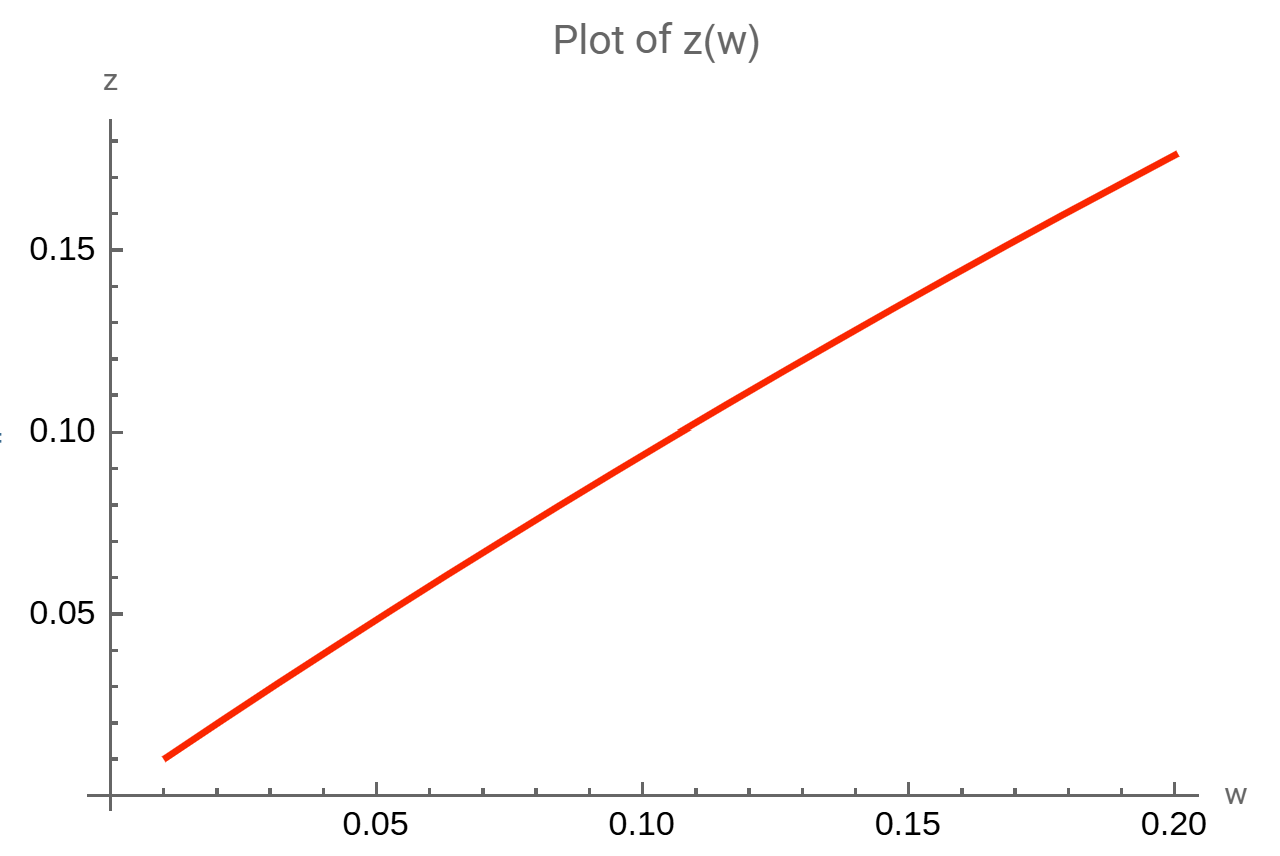
\includegraphics[width=0.3\textwidth]{Q1Csmall.png} % Replace 'figure.jpg' with your image file
        \caption{Plot of $z(w)$ for $w$ small.}
        \label{fig:Q1Csmall}
    \end{figure}
    \begin{figure}[h]
        \centering
        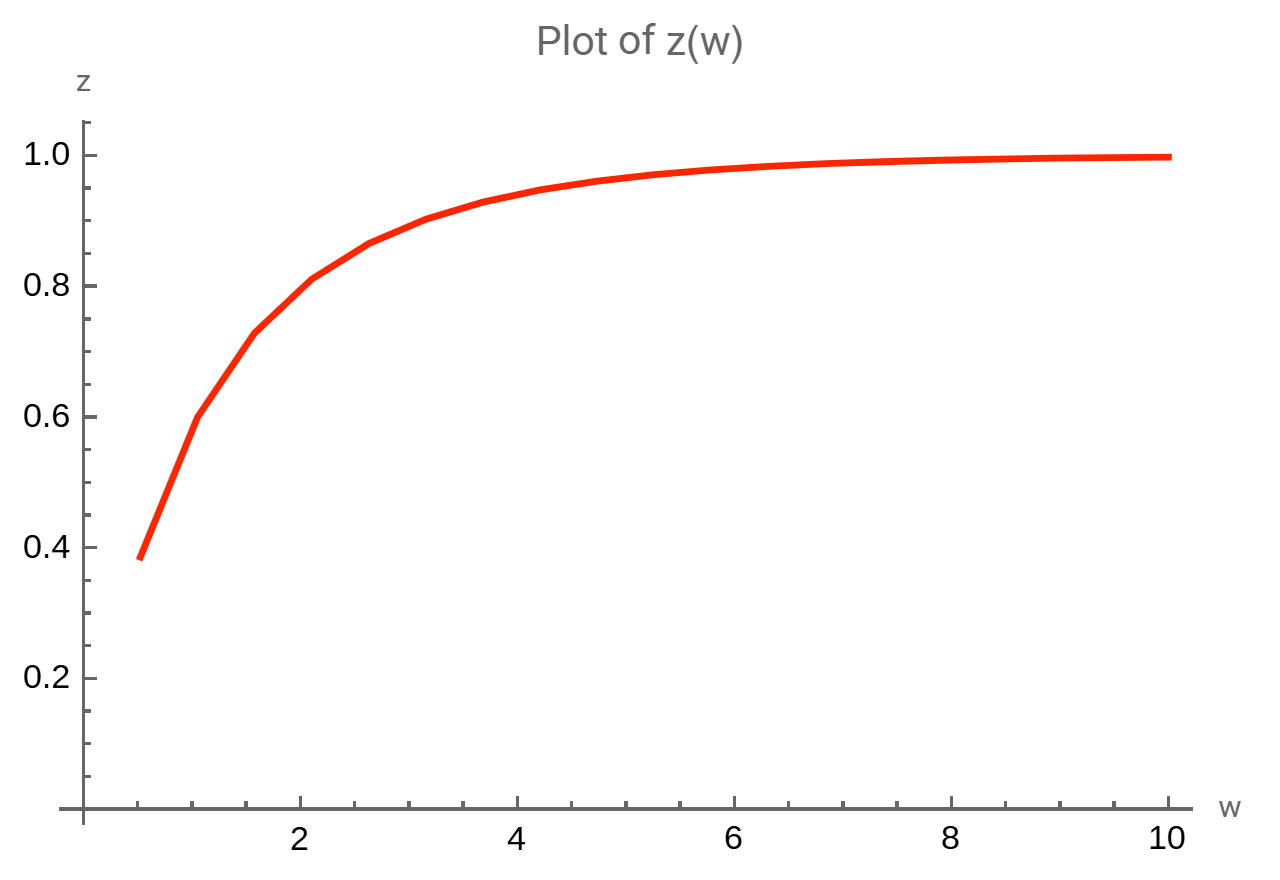
\includegraphics[width=0.3\textwidth]{Q1C.png} % Replace 'figure.jpg' with your image file
        \caption{Plot of $z(w)$ for $w$ large.}
        \label{fig:Q1C}
    \end{figure}
    The maximum value of $z$ is 1, and for small values of $w$, the 
    value is linear. 
\end{proof}

\textbf{(D) Small $w$: power series approach}

(i) Write $w$ as a power series in $z$ to order $z^3$.

(ii) Write $z$ in terms of $w$ as another power series solution
\begin{equation}\label{eqn:1D}
z = a_0 + a_1w + a_2w^2 + \dots
\end{equation}
and identify the coefficients $a_0$, $a_1$, and $a_2$ by matching the $w^0$, $w^1$, and $w^2$ terms order by order.

\begin{proof}[Solution]
    Using the taylor series expansion, we can easily solve for $w(z)$. 
    \begin{equation}
        w(z) \ = \ z + \frac 2 3 z^2 + \frac 1 2 z^3 + O(z^4)
    \end{equation}
    To solve for $z(w)$, we first observe that $z(0) = 0$ which implies 
    $a_0 = 0$. Plugging in to \eqref{eqn:Q1wzrelation}, we obtain the follwing. 
    \begin{eqnarray}
        w \ = \ 
        a_1 w + \left(
            \frac {2 a_1^2} 3 + a_2
        \right)w^2 + 
        \left(
            \frac {a_1^3} 2 + \frac {4a_1 a_2}3 + a_3
        \right)w^3 + O(w^4)
    \end{eqnarray}
    In order for the identity to hold, the coefficients of 
    $w^2, w^3$ must equal to zero. 
    \begin{eqnarray}
        (a_1, a_2, a_3) \ = \ \left(
            1, -\frac 2 3, \frac 7 {18}
        \right)
    \end{eqnarray}
\end{proof}


\textbf{(E) Small $w$: successive approximations approach}

(i) Re-write your equation for part C(i) as $z = w + f(z)$ where $f(z) = O(z^2)$. By arguing that the correction terms are negligible to first order, you can obtain a solution $z_1$ which is correct to first order in $w$.

(ii) Use this first-order solution $z_1$ to find an estimate that is correct to second order: $z_2 = w + f(z_1)$.

\begin{proof}[Solution]
    We notice 
    \begin{eqnarray}\label{eqn:Q1E}
        z \ = \ w - \frac 2 3 z^2 + O(z^3)
    \end{eqnarray}
    and for the sake of approximation, we set $z_0 = w$ and obtain a 
    sequence $z_n$ by the recursive relation 
    \begin{eqnarray}
        z_{n + 1} \ = \ w - \frac 2 3 z_n^2. 
    \end{eqnarray}
    Here is the first 3 terms of $z_n$ for $w = .6$. 
    \begin{eqnarray}
        (z_0, z_1, z_2, z_3) \ = \ (.6, .36, .51, .42)
    \end{eqnarray}

    
\end{proof}

\textbf{(F)} We can also use successive approximations to analyze the range equation for \textit{large} $w$. Start with the substitutions $z = 1 - e^{-\zeta}$, $\chi = w/2 + 1$. Use the method of successive approximations to discover how $\zeta$ depends on $\chi$. Note that for large $w$, $\chi$ and therefore $\zeta$ are also large. This is not a simple power series, so stop after the first iteration.

\begin{proof}[Solution]
The value of $w = 100$ yields $\chi = 51$. 
    It is straightforward to obtain 
    \begin{eqnarray}
        \zeta \ = \ 2 - \frac 2 \chi + \frac 2 3 \zeta^3
    \end{eqnarray}
    and we set up 
    \begin{eqnarray}
        \zeta_0 \ = \ 2 - \frac 2 \chi \ \approx \ 1.96. 
    \end{eqnarray}
    and compute the next value of $\zeta_n$. 
 \begin{eqnarray}
        \zeta_1 \ = \ 2 - \frac 2 \chi + \frac 2 3 \zeta_0^3 \approx 6.97
    \end{eqnarray}
    Recover the value of $z$ from $\zeta$. 
    \begin{eqnarray}
        z_1 \ = \ 1-e^{-\zeta} \ \approx \ 1.00
    \end{eqnarray}
\end{proof}

\textbf{(G)} Combine the results of (E) and (F) as plots on the same graph with the values in (C). \textit{Show} may be helpful. Finally, rewrite these approximations in terms of the lengths $R$, $R_{vac}$, and $R_{\infty}$.
\begin{proof}[Solution]
The plot below highlights the two approximations we made. 
\begin{figure}[h]
    \centering
    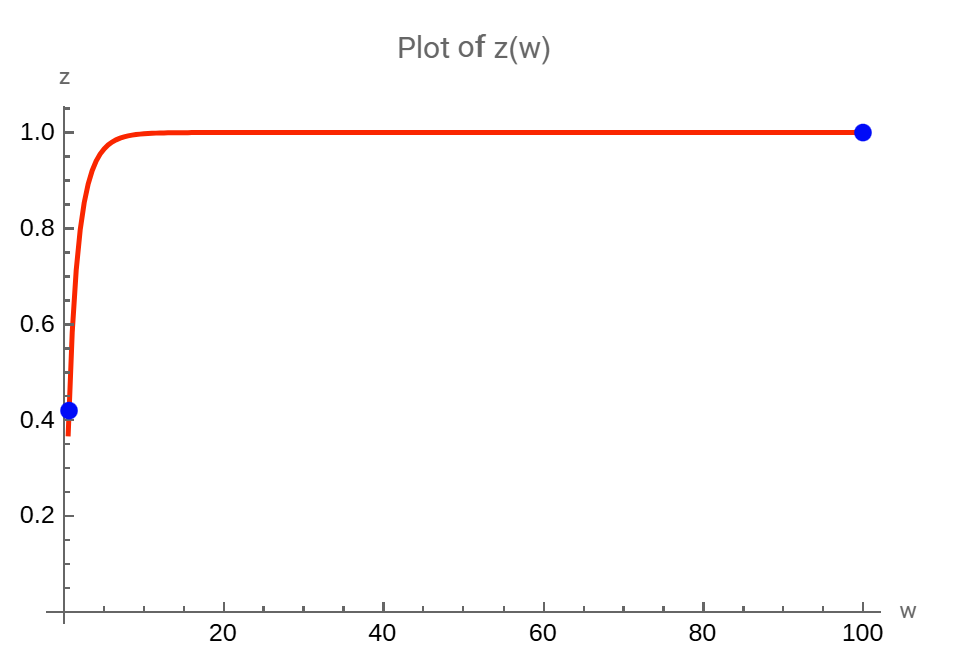
\includegraphics[width=0.8\textwidth]{Q1Dlarge.png} % Replace 'figure.jpg' with your image file
    \caption{Plot with approximations highlighted in blue }
    \label{fig:example}
\end{figure}

From \eqref{eqn:Q1E}, ignoring the error term for small $z$ and 
rewriting $z, r$ as ratios of $R$s, we obtain the follwing. 
\begin{eqnarray}
    R \ =\ R_{\rm vac} - \frac 2 3 \frac{R^2}{R_\infty}
\end{eqnarray}
\end{proof}

\section{Problem 2}

\textbf{t2.35}

(a) Fill in the details of the arguments leading from the equation of motion (2.52) to Equations (2.57) and (2.58) for the velocity and position of a dropped object subject to quadratic air resistance. Be sure to do the two integrals involved. (The results of Problem 2.34 will help.)

(b) Tidy the two equations by introducing the parameter $\tau = \frac{v_{\text{ter}}}{g}$. Show that when $t = \tau$, $v$ has reached 76\% of its terminal value. What are the corresponding percentages when $t = 2\tau$ and $t = 3\tau$?

(c) Show that when $t \gg \tau$, the position is approximately $y \approx v_{\text{ter}} t + \text{const}$. \textit{[Hint: The definition of $\cosh x$ (Problem 2.33)]}


\begin{proof}[Solution for a]
    We present two $\tanh(x)$ related formulas before providing the solution. 
    \begin{eqnarray}\label{eqn:tanhIntegral}
        \arctan(ui)  \ = \ i \textnormal{arctanh}(u) \nonumber\\ 
        \int_{0}^x \frac {du}{1 - u^2} \ = \ \textnormal{arctanh}(u) 
    \end{eqnarray}
    The first formula follows directly from the definition of 
    $\tanh(x)$, and the second formula can be deduced from the first 
    formula, and the well-known integral, 
    \begin{eqnarray}
        \int_0^x \frac {du}{1 + u^2} \ = \ \arctan(x) 
    \end{eqnarray}

    Move on to solve the problem. We start from 
    \begin{equation}
        m \frac {dv}{dt} \ = \ mg - cv^2
    \end{equation}
    and solve for $gdt$. Under the substitution 
    \begin{eqnarray}
        \widetilde v \ = \ \frac v {v_{\rm ter}}
    \end{eqnarray}
    it is not hard to see 
    \begin{eqnarray}
        \frac {v_{\rm ter} }{
            1 - \widetilde v^2
        } d \widetilde v\ = \ gdt.
    \end{eqnarray}
    We integrate both sides. \eqref{eqn:tanhIntegral} comes to the rescue. 
    We also assume that the object starts from rest, so $\widetilde v_0 = v_0 = 0$. 
    \begin{eqnarray}
        v_{\rm ter} \left[
            \textnormal{arctanh}(x)
        \right]_{0}^{\widetilde v} \ = \ 
        v_{\rm ter} \textnormal{arctanh}\left(
            \frac v {v_{\rm ter}}
        \right) \ = \ gt
    \end{eqnarray}
    Solve for $v$ and expres $\tanh$ as a fraction. 
    \begin{eqnarray}
        v \ = \ v_{\rm ter} \tanh \left(
            \frac {gt} {v_{\rm ter}}
        \right)
        \ = \ 
        v_{\rm ter} \frac{
            \sinh(gt/v_{\rm ter}) 
        }{
            \cosh(gt/v_{\rm ter})
        }
    \end{eqnarray}
    We know that $v = \frac {dy}{dt}$. Integrating both sides 
    by $t$ yields the desired answer. The u-subsitution $u = \cosh(gt/v_{\rm ter})$
    is convinient. 
    \begin{eqnarray}
        \int_0^T \frac {dy}{dt} dt \ = \ 
        \int_0^T 
        v_{\rm ter} \frac{
            \sinh(gt/v_{\rm ter}) 
        }{
            \cosh(gt/v_{\rm ter})
        }dt \ = \ 
        \int_0^{\cosh(gT/v_{\rm ter})} \frac {v_{\rm ter}^2} g \frac {du} u
         \nonumber \\ 
        \ = \ y(T) \ = \  \frac {(v_{\rm ter})^2} g \ln (\cosh(gt/v_{\rm ter}))
    \end{eqnarray}
\end{proof}

\begin{proof}[Solution for b]
    Equation (t2.56), (t2.58) converts to the following. 
    \begin{eqnarray}
        \tau \textnormal{arctanh}\left(
            \frac v {g\tau}
        \right) \ = \ t \\ 
        y \ = \ \tau^2 g \ln\left[
            \cosh\left(
                \frac t \tau
            \right)
        \right]
    \end{eqnarray}
    A useful identity can be salvaged from the first equation. 
    \begin{eqnarray}
        \frac v {v_{\rm ter}} \ = \ \tanh\left(\frac t \tau\right)
    \end{eqnarray}
    The identity gives the fractional velocity at time $t$. Computationally, 
    we find 
    \begin{eqnarray*}
        \tanh(1) \ = \ .76 \\ 
        \tanh(2) \ = \ .96 \\ 
        \tanh(3) \ = \ .99 
    \end{eqnarray*}
    which implies 
    \begin{eqnarray*}
        v(\tau) \ = \ .76 v_{\rm ter} \\ 
        v(2\tau) \ = \ .96 v_{\rm ter}\\
    v(3\tau) \ = \ .99v_{\rm ter}
    \end{eqnarray*}
\end{proof}

\begin{proof}[Solution for c]
    For $x \gg 1$, $\cosh(x) \approx e^x / 2$. With this in mind, 
    we proceed from the identity obtained in b. 
    \begin{eqnarray}
        y \ = \ 
        \tau^2 g \ln \left[
            \cosh\left(
                \frac t \tau
            \right)
        \right] \ \approx \  
        \tau^2 g \ln\left(
            \frac{e^{t/\tau}} 2
        \right) \ = \  
        v_{\rm ter} g - v_{\rm ter} \tau \ln(2)
    \end{eqnarray}
\end{proof}

\textbf{t2.44}
 To get an accurate trajectory for a projectile, one must often take account of several complications. For example, if a projectile goes very high then we have to allow for the reduction in air resistance as atmospheric density decreases. To illustrate this, consider an iron cannonball (diameter 15 cm, density 7.8 g/cm$^3$) that is fired with initial velocity 300 m/s at 50 degrees above the horizontal. The drag force is approximately quadratic, but since the drag is proportional to the atmospheric density and the density falls off exponentially with height, the drag force is 
\[
f = c(y)v^2
\]
where \(c(y) = \gamma D^2 \exp(-y/\lambda)\) with \(\gamma\) given by (2.6) and \(\lambda \approx 10,000 \text{ m}\).

\textbf{(a)} Write down the equations of motion for the cannonball and use appropriate software to solve numerically for \(x(t)\) and \(y(t)\) for \(0 \leq t \leq 3.5 \text{ s}\). Plot the ball’s trajectory and find its horizontal range.

\textbf{(b)} Do the same calculation ignoring the variation of atmospheric density (that is, setting \(c(y) = c(0)\)), and yet again ignoring air resistance entirely. Plot all three trajectories for \(0 \leq t \leq 3.5 \text{ s}\) on the same graph. You will find that in this case air resistance makes a huge difference and that the variation of air resistance makes a small, but not negligible, difference.


\begin{proof}[Solution]
    Other than the quantities provided in the problem statement, 
    we have to specify the mass of the projectile and the initial velocity. 
    The mass can be computed by density times volume. The initial 
    velocity is given in polar coordinates, and can be easily converted 
    by basic trignometry. 
    \begin{equation}
        m \ =\ \rho V \ = \ \frac 1 6 \rho D^3 \pi 
        \textAnd 
        (v_{x0} , v_{y0}) \ = \ (v_0\cos(\theta_0), v_0 \sin(\theta_0))
    \end{equation}
    Also, remember to convert all quantities to mks units. 
    \begin{eqnarray}
        (D, \rho) \ = \ (.15m, 7800kg/m^3)
    \end{eqnarray}

    We set the vector pointing downwards to be our positive $y$ direction. 
    Then, we obtain the folling set of differential equations for the velocity. 
    \begin{eqnarray}
        m\dot v_x \ = \ -c(y) \sqrt{v_x^2 + v_y^2} v_x \nonumber \\ 
        m\dot v_y \ = \ mg - c(y) \sqrt{v_x^2 + v_y^2} v_y
    \end{eqnarray}
    
    This gives motivation to the following numerical approximation on \ref{fig:Q3code}. 
    With slight modification, we account for constant drag and the 
    case without drag and obtain the plot in Figure \ref{fig:Q3AllProjectiles}
   .  
    \begin{figure}[h]
        \centering
        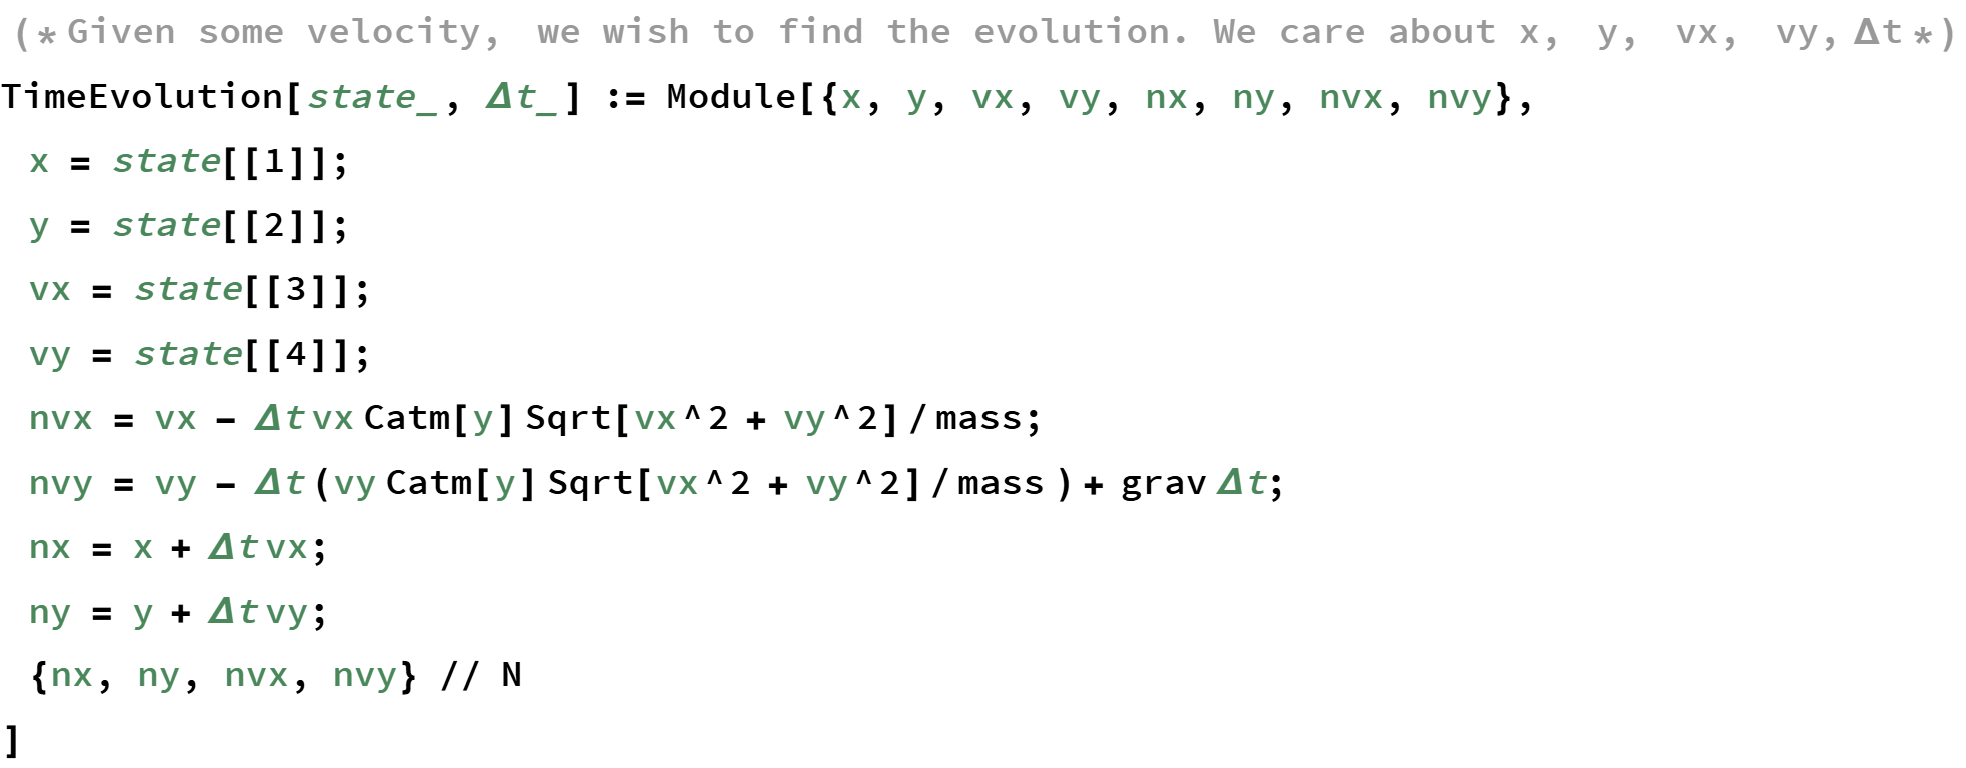
\includegraphics[width=0.8\textwidth]{Q3Code.png} % Replace 'figure.jpg' with your image file
        \caption{Mathematica code for the numerical approximation}
        \label{fig:Q3code}
    \end{figure}
    \begin{figure}[h]
        \centering
        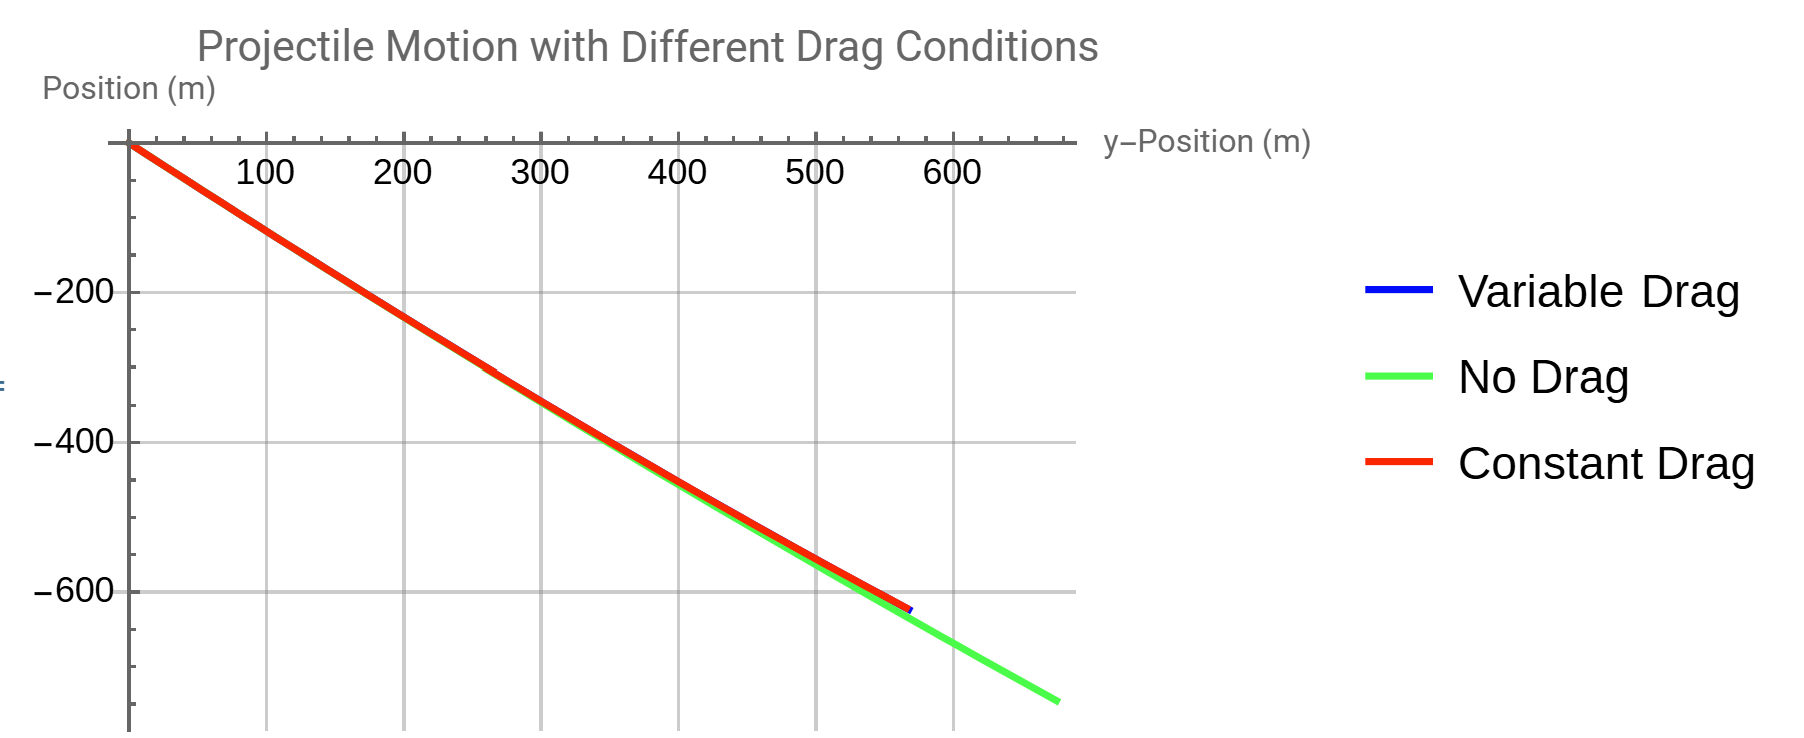
\includegraphics[width=0.8\textwidth]{Q3AllProjectiles.png} % Replace 'figure.jpg' with your image file
        \caption{Mathematica plot of all three projectiles}
        \label{fig:Q3AllProjectiles}
    \end{figure}
    
    
\end{proof}

\section{Problem 3} 
\textbf{Characteristic Quantities and Dimensionless Equations}

In problems (1) and (2) above you were handed ‘characteristic quantities’ that allowed you to simplify the equations. But, such quantities will often reveal themselves purely by dimensional arguments. One way to find them is to non-dimensionalize the equations as we will here.

\subsection*{(A)} 
Imagine a particle moves horizontally (perhaps skidding on a frictionless plane), such that it feels both linear and quadratic drag. Starting from Taylor’s Eq. (2.1), recast the equation of motion in dimensionless form. To do so, define a dimensionless velocity \( V = v/v_c \) and time \( T = t/t_c \), and let the mathematics inform ‘good’ choices for \( v_c \) and \( t_c \). You should find
\[
\frac{dV}{dT} = -V - V^2.
\]
What characteristic quantities do you find? Is there more than one reasonable choice? Comment on their physical relevance; note how much you can learn without solving anything, purely by dimensional analysis!

\subsection*{(B)} 
Solve (by hand) the scaled differential equation for \( V(T) \). Comment on limiting cases; show that the solution reduces to the behavior for linear or quadratic drag in the appropriate limits.

\subsection*{(C)} 
Notice that here we have arrived at a ‘universal’ solution. That is, a plot of \( V(T) \) could be modified to account for any possible choice of system parameters just by scaling the axes appropriately. What happens if we modify the problem to have our particle \textit{falling} in air, i.e.
\[
m \frac{dv}{dt} = mg - bv - cv^2.
\]
Your first instinct might be to say that this should behave like Taylor’s Eq. (2.14) for \( c \ll b \), and like (2.52) for \( b \ll c \), but this is meaningless (why?). Sort out an intelligent way to think about limiting cases, and discuss these cases. There is almost certainly more than one way to go about this; anything reasonable is fine. You needn’t try to solve the differential equation, but do find the terminal velocity in the various limits. Do your results agree with Taylor’s? Is there a universal solution?

\begin{proof}[Solution for a, b]
    We consider a particle that expereinces both linear and quadradic 
    drag. Assume the motion to be restricted in one dimension. Drawing 
    the free body diagram, we write out a differential equation for 
    the velocity.
    \begin{eqnarray}
        m \frac {dv}{dt} \ = \ -(bv + cv^2)
    \end{eqnarray}
    If we set 
    \begin{eqnarray}\label{eqn:subst}
        v_c \ = \ b/c \textAnd t_c \ = m/ b \\ 
        V \ := \ \frac v {v_c} \textAnd 
        T \ := \ \frac t {t_c}
    \end{eqnarray}
    \footnote{
        It is also possible to do dimensional analysis on $v_c$ and 
        $t_c$ and confirm that they are both velocity and time. 
        $[v_c] = [b]/[c] = N/(m/s)/(N/(m^2/s^2)) = m/s$ and 
        $[t_c] = [m]/[b] = kg/[N/(m/s)] = kg/[kg/s] = s$. 
    }\footnote{
        Also, this susbstitution is unique to obtain \eqref{eqn:dimensionLess} without 
        constants. It is possible to choose other quantities to get a dimensionless 
        equation, but there will be constants lingering in the equation. 
    }
    we can rewrite the differential equation in dimensionless quantitues $V, T$. 
    \begin{align}
        dt \ = \ t_c dT  \nonumber \\ 
        dv \ = \ v_c dV  \nonumber \\ 
        m\frac {v_c}{t_c} \frac {dV}{dT} \ = \ -v_c b V - (v_c)^2 c V^2 \nonumber \\ 
        \frac m {t_c}\frac {dV}{dT} \ = \ -bV -v_c cV^2 \nonumber \\ 
        \label{eqn:dimensionLess}\frac {dV} {dT} \ = \ -(V + V^2)
    \end{align}
    This is a separable equation, a solution for $V(T)$ can be easily 
    derived by u-substitution. Suppose the initial velocity of the object is 
    $v_0$. 
    \begin{eqnarray}
        \int_{V_0}^{V} \frac {dV}{V^2 + V} \ = \ 
        \int_{0}^{T} dT  
    \end{eqnarray}
    Under the subsitution, $x = 1+1/V$, we integrate the lefthand side. 
    \begin{align}
         \int_{V}^{V = V_0} \frac {dx}{x} \ = \ T\\ 
            \ln(x)\bigg|_{x = 1 + 1/V}^{1 + 1/V_0} \ = \ T\\
            V \ = \ \frac 1 {e^T(1 + 1/V_0) - 1} \label{eqn:exactSol}
    \end{align}
    Now we consider the limiting case. If $b \gg 1$, then $T = t/t_c = bt/m$ 
    will be large. It is reasonable to ignore the $-1$ in the denominator. 
    \begin{eqnarray}
        V \ \approx \ \frac {e^{-t}} {1 + 1/V_0}
    \end{eqnarray}
    and this equation turns out to be the solution of the case 
    without quadratic drag, i.e.
    \begin{equation}
        \frac {dV} {dT} = -V. 
    \end{equation}
    If $b \ll 1$ and $c/b \gg 1$, then we can assume $T$ small and substitute 
    $e^T$ with its Taylor expansion. We focus on the denominator of 
    \eqref{eqn:exactSol}. 
    \begin{align}
        \left(
            1 + T
        \right)(1 + 1/V_0) - 1 \ = \  
        T + 1/V_0 + T/V_0 \ \approx \ T + 1/V_0 
    \end{align}
    The last approximation follows from the observation that 
    $T/V_0\propto b/c^2$ and that $b/c^2$ is small. Thus, \eqref{eqn:exactSol} 
    is rewritten as 
    \begin{eqnarray}
        V \ = \ \frac 1 {T + 1/V_0}
    \end{eqnarray} and this equation turns out to be the solution of the case 
    without linear drag, i.e.
    \begin{equation}
        \frac {dV} {dT} = -V^2. 
    \end{equation}
\end{proof}
\begin{proof}[Solution for c]
    We first compute the teminal velocity. When the object reaches 
    terminal velocity, then $\dot v = 0$. Hence, for all cases, we have 
    \begin{eqnarray}
        0 \ = \ -bv_{\rm ter} -c(v_{\rm ter})^2 + mg
    \end{eqnarray} 
    andy by the quadratic equation, we get the terminal velocity which is 
    \begin{eqnarray}
        v_{\rm ter} \ = \ \frac{
            \sqrt{b^2 + cmg} - b
        }{2c}
    \end{eqnarray}
    where the negative root is ignored; it is physically impossible 
    that the object moves in the same direction of the drag. 

    We have shown in part b) that for $b\gg c$, we can ignore quadradic drag. 
    In this case, from our solution of 
    \begin{eqnarray}\label{eqn:linWoDrag}
        m \dot v \ = \ - bv
    \end{eqnarray}
    we can solve
    \begin{align}\label{eqn:linWDrag}
        m \dot v \ = \ mg - bv.
    \end{align}
    Suppose \eqref{eqn:linWoDrag} has a solution $v^*(t)$. We claim that 
    $v(t) = v_{\rm ter} + v^*(t)$ solves \eqref{eqn:linWDrag}. 
    Taking the time derivative on the lefthand side with drag, we obtain
    \begin{eqnarray}
        m \frac {dv(t)}{dt} \ = \ m \frac {dv^*(t)}{dt} \ = \ m\dot{v^*} = -bv^*(t) 
    \end{eqnarray}
    and we compute the righthand side to obtain the same expression. 
    \begin{align}
        mg - b(v_{\rm ter}+v^*(t)) \ = \ -bv^*(t)
    \end{align}

    As for the other limiting case, $c \gg b$, we have shown that we 
    can ignore the linear drag. Under the same substitution as in \eqref{eqn:subst}, 
    we write out a approximated differentail equation. 
    \begin{equation}
        \dot V \ = \ -V^2 + \xi
    \end{equation}
    The quantity $\xi$ is the correction incurred by gravity. 
    \begin{eqnarray}
        \xi \ = \ \frac {mg}{v_c}
    \end{eqnarray}
    The equation is separable, and using the arctanh formula, 
    we obtain a closed form expression for $V$. 
    \begin{align}
        V \ = \ \sqrt{\xi} \left[\textnormal{arctanh}\left(
            \frac {V_0}{\xi} + \xi T
        \right)\right]
    \end{align}

    \begin{remark}

So we consider two terminal velocities. The terminal velocity is determined by:

\[
mg - b v_{\text{lin}} - c v_{\text{quad}}^2 = 0
\]

The terminal velocity without quadratic decay is:

\[
v_{\text{lin}} = \frac{mg}{b}
\]

The terminal velocity with quadratic decay is:

\[
v_{\text{quad}} = \sqrt{\frac{mg}{c}}
\]

If \(v_{\text{lin}} \gg v_{\text{quad}}\), then we conjecture that quadratic decay can be ignored:

\[
\frac{mg}{b} \gg \sqrt{\frac{mg}{c}}
\]

So,

\[
\frac{\sqrt{mg}}{b} \cdot \sqrt{c} \gg 1
\]

If \(v_{\text{lin}} \ll v_{\text{quad}}\), then:

\[
\frac{\sqrt{mg}}{b} \cdot \sqrt{c} \ll 1
\]

So instead of comparing \(c, b\), we can consider the magnitude of the dimensionless quantity:

\[
\sqrt{\frac {mgc}{b^2}} = \chi
\]
\end{remark}
\end{proof}

\section{Problem 4}
\textbf{2.52}
The transverse velocity of the particle in Sections 2.5 and 2.7 is contained in (2.77), since 
\[
\eta = v_x + iv_y.
\]
By taking the real and imaginary parts, find expressions for \( v_x \) and \( v_y \) separately. Based on these expressions describe the time dependence of the transverse velocity.

\begin{proof}[Solution]
    We remember that the solution for $\eta$ is 
    \begin{eqnarray}
        \eta \ = \ A e^{\theta - \omega t}
    \end{eqnarray}    
    where $A$ is some real number and $\theta$ is some angular offset. 
    $\omega$ is called the \textbf{Cyclotomic Frequency} and is defined as 
    \begin{eqnarray}
        \omega \ = \ \frac{qB} m
    \end{eqnarray}
    Expanding the complex exponential by trignometric functions, we 
    obtain $v_x, v_y$. 
    \begin{eqnarray}
        \eta \ = \ v_x + iv_y \ = \ A e^{i \omega t} \ = \ A \cos (\theta - \omega t) + A
        i\sin(\theta -\omega t)\nonumber\\ 
        (v_x, v_y) \ = \ (A\cos(\omega t - \theta), -A\sin(\omega t - \theta))
    \end{eqnarray}
    Note that the magnitude of the \textbf{transverse velocity} i.e. the vector 
    $v_x\hat x + v_y \hat y$ has a constant magnitude, and the direction rotates 
    clockwise at the cyclotomic frequency. 
\end{proof}

 \textbf{t2.54}
In Section 2.5 we solved the equations of motion (2.68) for the transverse velocity of a charge in a magnetic field by the trick of using the complex number 
\[
\eta = v_x + i v_y.
\]
As you might imagine, the equations can certainly be solved without this trick. Here is one way:

\begin{itemize}
    \item[(a)] Differentiate the first of equations (2.68) with respect to \( t \) and use the second to give you a second-order differential equation for \( v_x \). This is an equation you should recognize [if not, look at Equation (1.55)] and you can write down its general solution. Once you know \( v_x \), (2.68) tells you \( v_y \).
    
    \item[(b)] Show that the general solution you get here is the same as the general solution contained in (2.77), as disentangled in Problem 2.52.
\end{itemize}


\begin{proof}[Solution]
    We wish to solve the following system of differential equations. 
    \begin{eqnarray}
        \dot v_x \ = \ \omega v_y \\ 
        \dot v_y \ = \ -\omega v_x
    \end{eqnarray}
    Taking the time derivative of the first equation and making the subsitution, 
    we obtain a second order equation on $v_x$. 
    \begin{eqnarray}
        \ddot v_x \ = \ \omega \dot v_y \ = \ -\omega^2 v_x
    \end{eqnarray}
    The solution for this second order is the well-known sum of trignometric functions. 
    From the solution of $v_x$, we also find $v_y$ using the second equation. 
    \begin{eqnarray}
        v_x \ = \ A \cos(\omega t) + B\sin(\omega t) \\ 
        v_y \ = \ B\cos(\omega t) - A \sin(\omega t)
    \end{eqnarray}
    It remains to show that this equation is somehow expressible in 
    the form of $v_x = C\cos(\omega t - \theta)$. Use the sum of cosines formula. 
    \begin{eqnarray}
        v_x \ = \ C\cos(\omega t - \theta) \ = \ 
        C \cos(\omega t) \cos(\theta) + C \sin(\omega t)\sin(\theta)
    \end{eqnarray}
    And since $\theta$ is a constant offset angle, the substitution 
    $C\cos(\theta) = A$, $C\sin(\theta) = B$ shows equivalence of the two 
    solutions. Same goes for $v_y$ using the difference of sines formula. 
    
\end{proof}


\section{Problem 5}
\begin{proof}[Solution]
    We approach the problem in a slightly general angle. Consider 
    a system of two masses $M, m$ moving in some constant velocity. 
    At some point, the mass $m$ departs mass $M$ at a relative velocity $\vec u$. 
    To qualify, after the departure, the speed of mass $m$ measured with 
    respect to mass $M$ is $u$. 
    Frames that move in constant velocity are inertial. Thus, the 
    two masses can be considered stationary. Using conservation of momentum, 
    we derive the velocity change of the large mass. 
    \begin{eqnarray}
        \Delta v_M M + (\Delta v_M + u) m \ = 0 \nonumber \\ 
        \Delta v_M \ = \  -\frac m {M + m} \vec u 
    \end{eqnarray}
    So the change of velocity of the large mass is $\vec u$ multiplied 
    by the fraction of the mass over the combined mass. Continuously applying this 
    proposition, we obtain the following results. 
    \begin{eqnarray}
    \vec v_{j = 1}  & =  & -\frac {2m} {M + 2m} \vec u \\ 
    \vec v_{j = 2} & = & -\left(
        \frac m {M + m} + \frac m {M + 2m}
    \right)\vec u 
\end{eqnarray}\footnote{Taking the magnitude, this result concurs with what is listed in the problemset}
Upon inspection $\vec v_{j = 1}$ is larger than $\vec v_{j = 2}$ since 
$\frac m {M + m} < \frac m M$. 
For $N$ masses leaving $M$, we have the following formula. 
\begin{eqnarray}
    \vec v_{j = n} & = & -\left(\sum_{i = 1}^N \frac m{M + im} \right) \vec v/
\end{eqnarray}
We set $Nm$ to be constant and send $N \rightarrow \infty$. Convert 
the sum to an integral. The substitution $m = dx, im = x$ comes in handy. 

\begin{equation}
    \vec v_{j=\infty} \ = \ 
     -\left(\int_{x = 0}^{Nm} \frac {dx}{M + x} \right) \vec v \ = \ 
     -\left[
        \ln(M + x)
     \right]_0^{Nm}\vec v \ = \ \ln\left(
        \frac {M} {M + Nm}
     \right)\vec v
\end{equation}

This equation concurs with (t3.4). 

\end{proof}



\end{document}